\documentclass[11pt, oneside]{article} 
\usepackage{geometry}
\geometry{letterpaper} 
\usepackage{graphicx}
	
\usepackage{amssymb}
\usepackage{amsmath}
\usepackage{parskip}
\usepackage{color}
\usepackage{hyperref}

\graphicspath{{/Users/telliott_admin/Dropbox/Tex/png/}}
% \begin{center} 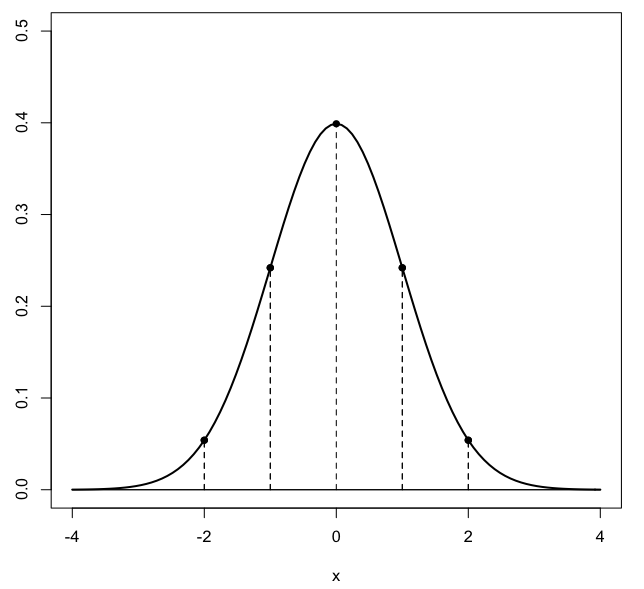
\includegraphics [scale=0.4] {gauss3.png} \end{center}

%break
\title{Difference quotients}
\date{}

\begin{document}
\maketitle
\Large

In this chapter we look at the geometric interpretation of the derivative --- which is the traditional  way to begin calculus.  The general approach was developed by Fermat.

Think for a minute about a curve such as the one shown in the figure, corresponding to some unspecified function $f(x)$.
\begin{center} 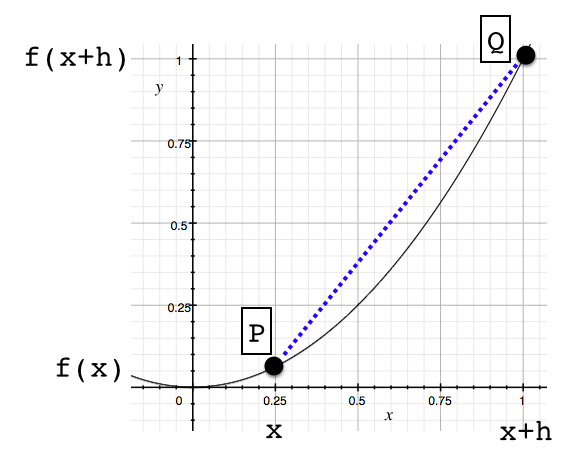
\includegraphics [scale=0.4] {diff_quotient.png} \end{center}

At an arbitrary point $P$ on the curve, for some value of $x$, we plot $y = f(x)$.  This is Descartes' genius idea.  The point on the graph of $f(x)$ at $x$ has coordinates $P=(x,f(x))$.  

Now consider a point $Q$ near $P$ but also on the curve, For the $x$-coordinate of $Q$, a small amount is added to $x$.  We might call that small amount $\Delta x$, but many authors use $h$, a simpler notation, and we will do so as well.  The value of the function at $x+h$ is $f(x+h)$ and so $Q$ has coordinates $Q=(x+h,f(x+h))$.

The slope of the (secant) line connecting $Q$ and $P$ is

\[  \frac{\Delta y}{\Delta x} = \frac{f(x+h) - f(x)}{x + h - x} = \frac{f(x+h) - f(x)}{h} \]

This is a famous quantity, it's called the \textbf{difference quotient}.

The goal of differential of calculus is to find the slope of the \emph{tangent} to the curve at the point $P$.  What we have is an expression for the slope of the secant line $PQ$, which is close but not quite the same thing.

To go from the secant to the tangent, we ask "what happens to this expression as $h$ gets smaller and smaller and approaches zero."  The second point where the secant meets the curve comes closer and closer to the first one.

\begin{center} 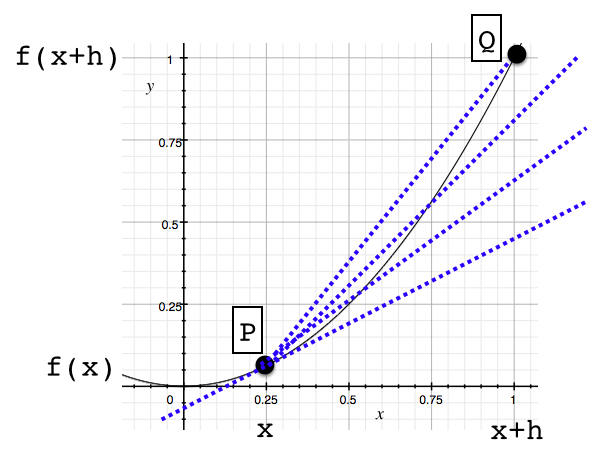
\includegraphics [scale=0.4] {diff_quotient2.png} \end{center}

In mathematical language, we say the slope of the tangent is equal to the limit of the difference quotient as $h$ tends to $0$:
\[  \lim_{h \to 0} \  \frac{f(x+h) - f(x)}{h} \]

We'll say a bit more about limits in the next chapter, but for the moment you can think about 
\[  \lim_{h \to 0} \]
as meaning, "substitute $h=0$ and see what happens to the expression of interest."

\subsection*{x squared}

Let's try a couple of examples and look for a pattern.
\[    f(x)=x^2  \]

For this function, we write that the difference quotient is
\[    \frac{(x+h)^2 - x^2}{h} \]
\[    = \frac{x^2 + 2xh + h^2 - x^2}{h} \]
\[    = \frac{2xh + h^2}{h} \]

Now divide by the denominator $h$
\[    = 2x + h \]
    
Finally, to get the slope of the tangent, we evaluate the limit
\[    \lim_{h \to 0} \  2x + h = 2x \]

In evaluating the limit, we ask:  what happens to this expression as $h$ approaches $0$.  In this case, it cannot actually reach zero, because then our previous step of dividing by $h$ would not be allowed.  But we let $h$ become really really small, and take advantage of the property of the limit which says that an expression can have a limit at $c$ even if it can't be evaluated at $c$ itself.

At every point on the curve $y=x^2$, the slope of the tangent line to the curve is $2x$.  So the slope at $x=0$ is $0$, and the slope at $x=2$ is $4$, and so on.

This process of computing the difference quotient and then finding the limit as $h \to 0$ is called "taking the derivative."  It produces an expression which is called the derivative of $y$ with respect to $x$, in this case
\[   \frac{dy}{dx} = 2x \]
and we can interpret this as the slope of the tangent to the curve of $f(x)$ at the point $x$.

Another useful shorthand uses the $f$ from $f(x)$.  We adopt the convention that the derivative of $f(x)$ can be written $f'(x)$.
\[    f'(x) = 2x \]
To be even more succinct we might write $y'$ for $f'(x)$.

If we repeat this exercise with a leading constant $a$ (that is, for $f(x) = ax^2$), we find that every term in the numerator of the difference quotient will contain $a$, and the final result will be $2ax$.  Constants just get carried through.

\subsection*{square root}

Now look at the square root:
\[  f(x)=\sqrt{x}, \ \ (x \ge 0) \]

The difference quotient for this function is
\[   \frac{\sqrt{x+h} - \sqrt{x}}{h} \]

Clean up the numerator by multiplying by the conjugate
\[    \frac{\sqrt{x+h} - \sqrt{x}}{h} \ \  \frac{\sqrt{x+h} + \sqrt{x}}{\sqrt{x+h} + \sqrt{x}} \]
\[    = \frac{x + h - x}{h \ (\sqrt{x+h} + \sqrt{x})} \]
\[    = \frac{h}{h \ (\sqrt{x+h} + \sqrt{x}) } \]
\[    = \frac{1}{\sqrt{x+h} + \sqrt{x}} \]

We evaluate the limit
\[    \frac{dy}{dx} = \lim_{h \to 0} \  \frac{1}{\sqrt{x+h} + \sqrt{x}} = \frac{1}{2\sqrt{x}} \]

\subsection*{inverse}

Consider the inverse function
\[   f(x)=1/x, \ \ (x \ne 0) \]
\[    \frac {  \frac{1}{x+h} - \frac{1}{x}  }  {h} \]

Clean up the numerator
\[    \frac {  \frac{1}{x+h} - \frac{1}{x}  }  {h} \ \  \frac{(x)(x+h)}{(x)(x+h)} \]
\[    = \frac {x - (x+h)}  {h\ (x) \ (x+h)} \]
\[    = \frac {-h}  {h\ (x) \ (x+h)} \]
\[    = -\frac {1}  {(x) \ (x+h)} \]

We evaluate the limit:
\[    \lim_{h \to 0} \  -\frac {1}  {(x) \ (x+h)} \]
\[ \frac{dy}{dx} = - \frac{1}{x^2} \]

There's a pattern here.  We will use the notation $f'(x)$ to indicate the slope of the curve $f(x)$ at $x$
\[       f(x) = x^2 \ \ \Rightarrow \ \  f'(x) = 2x \]
\[       f(x) = \sqrt{x} = x^{1/2}\ \ \Rightarrow \ \  f'(x) = \frac{1}{2}x^{-1/2} \]
\[       f(x) = \frac{1}{x} = x^{-1} \ \ \Rightarrow \ \  f'(x) = -\frac{1}{x^2} = -x^{-2} \]

The general formula is
\[       f(x) = x^n \ \ \Rightarrow \ \  f'(x) = nx^{n-1} \]

This is easily proved (for integer $n$) using the binomial expansion for $(x + h)^n$ for integral $n$ ($n \in 1,2, \dots$).  We need only the first three terms:
\[         (x + h)^n = x^n + n x^{n-1} h + n\frac{(n-1)}{2}x^{n-2} h^2 + \dots  \]

The key point is that the last term shown and all subsequent terms contain powers of $h^2$ or higher.  

After division by $h$, for each of these terms there will remain one or more terms of $h$, and in the limit $\lim_{h \to 0}$ these become zero.
\[            \lim_{h \to 0} \ \frac{(x+h)^n - x^n}{h}  \]
\[            = \lim_{h \to 0} \ \frac{x^n + n x^{n-1} h + n\frac{(n-1)}{2} \ x^{n-2} h^2 + \dots - x^n}{h}  \]
\[            = \lim_{h \to 0} \ \frac{n x^{n-1} h + n\frac{(n-1)}{2}  \ x^{n-2} h^2 + \dots}{h}  \]
\[            = \lim_{h \to 0} \ n x^{n-1} + n\frac{(n-1)}{2}  \ x^{n-2} h + \dots  \]
\[            = n x^{n-1}  \]

Another question is what to do with a sum or difference of polynomials, such as 
\[            f(x) + g(x)    \]
If you write out the difference quotient
\[      \frac{ f(x+h) - f(x) + g(x+h) - g(x)}{h}  \]

everything can be exactly as before, just grouping all terms with $f(x)$ and those with $g(x)$ separately. 
\[      [f(x) + g(x)]' = f'(x) + g'(x)  \]

We showed above by computing the difference quotient directly that
\[      f(x) = \sqrt{x}  \] 
\[      f'(x) = \frac{1}{2\sqrt{x}}  \]

Here is another approach to the same problem.  Consider
\[      y = x^2  \]
\[      \frac{dy}{dx} = 2x  \]   
Solve for $x$ as a function of $y$:
\[      x = \sqrt{y}  \]
We can do algebra with \emph{differentials} (with some constraints):
\[      \frac{dy}{dx} \ \frac{dx}{dy} = 1  \]
\[      2 x \ \frac{dx}{dy} = 1  \]
\[      \frac{dx}{dy} = \frac{1}{2x} =\frac{1}{2 \sqrt{y}}  \]

In observing the inverse relationship, remember that $x$ and $y$ are related by the equation $y = x^2$.  For example, when $x=2$, $dy/dx = 2x = 4$.

Using the relationship $f(x)$, when $x=2$, $y=4$, and $dx/dy = 1/ 2 \sqrt{y} = 1/ 2 \sqrt{4} = 1/4$, which is indeed the inverse of $4$.

In this last section, after solving for $x$ as a function of $y$, $y$ is the \emph{independent} variable.  We can switch back to our usual notation:
\[      \frac{dy}{dx} =\frac{1}{2 \sqrt{x}}  \]

\subsection*{problem}

I found the following problems on the web.  They are great practice and show what kinds of problems this approach of differentiation can solve.  To prove:
\begin{center} 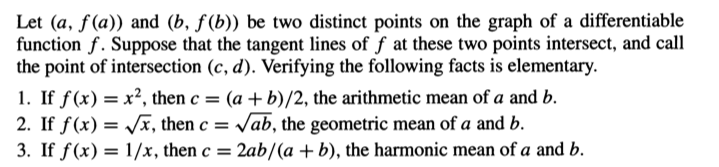
\includegraphics [scale=0.6] {mean_problem.png} \end{center}

\textbf{1}

Here is a diagram for the first one:
\begin{center} 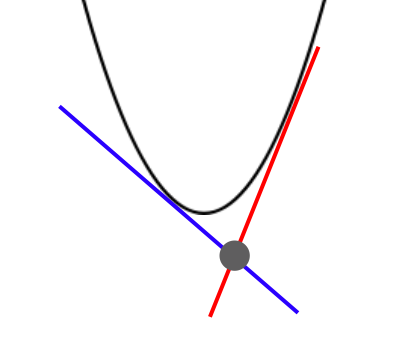
\includegraphics [scale=0.4] {two_lines.png} \end{center}
The claim is that the $x$-coordinate of the point will be half-way between the $x$-coordinates for the two points on the parabola.  We have:
\[ y = f(x) = x^2 \]
\[ y' = f'(x) = 2x \]

At $x = a$, the slope is $2a$ and the equation of a line through the point $(a, a^2)$ is
\[ y - a^2 = 2a(x - a) \]
At $x = b$, the equation is
\[ y - b^2 = 2b(x - a) \]
To see where the lines cross, we set the $y$'s to be equal, and solve for $x$:
\[ 2a(x - a) + a^2 = 2b(x - b) + b^2 \]
\[ 2ax - a^2 = 2bx - b^2 \]
\[ 2x(a - b) = a^2 - b^2 \]
\[ = (a + b)(a - b) \]
\[ x = \frac{1}{2} (a + b) \]
\textbf{2}

We have:
\[ y = f(x) = \sqrt{x} \]
\[ y' = f'(x) = \frac{1}{2 \sqrt{x}} \]

At $x = a$, the slope is $1/2 \sqrt{a}$ and the equation of a line through the point $(a, \sqrt{a})$ is
\[ y - \sqrt{a} = \frac{1}{2 \sqrt{a}} \ (x - a) \]
At $x = b$, the equation is
\[ y - \sqrt{b} = \frac{1}{2 \sqrt{b}} \ (x - b) \]
We set the $y$'s to be equal
\[ \frac{1}{2 \sqrt{a}} \ (x - a) + \sqrt{a} =  \frac{1}{2 \sqrt{b}} \ (x - b) + \sqrt{b} \]
and solve for $x$.  Multiply by $2 \sqrt{a}\sqrt{b}$
\[ (x - a)\sqrt{b} + 2a \sqrt{b} = (x - b) \sqrt{a} + 2 b \sqrt{a} \]
Multiply through and cancel
\[ x \sqrt{b} + a \sqrt{b} = x \sqrt{a} + b \sqrt{a} \]
\[ x(\sqrt{b} - \sqrt{a}) = b \sqrt{a} - a \sqrt{b} \]
\[ = \sqrt{a}\sqrt{b} (\sqrt{b} - \sqrt{a}) \]
\[ x = \sqrt{ab}\]

\textbf{3}

We have:
\[ y = f(x) = \frac{1}{x} \]
\[ y' = f'(x) = - \frac{1}{x^2} \]
At $x = a$, the slope is $-1/a^2$ and the equation of a line through the point $(a, 1/a)$ is
\[ y - 1/a = -\frac{1}{a^2} \ (x - a) \]
At $x = b$, the equation is
\[ y - 1/b = -\frac{1}{b^2} \ (x - b) \]
We set the $y$'s to be equal
\[  -\frac{1}{a^2} \ (x - a) + 1/a =  -\frac{1}{b^2} \ (x - b) + 1/b \]
and solve for $x$:
\[ (\frac{1}{b^2} - \frac{1}{a^2}) x = 2 ( \frac{1}{b} - \frac{1}{a} ) \]
\[ ( \frac{1}{b} + \frac{1}{a} ) x = 2 \]
\[ (a + b) x = 2ab \]
\[ x = \frac{2ab}{a + b} \]

\end{document}